\documentclass[pdftex,12pt,titlepage=false]{scrartcl}

\usepackage[table,dvipsnames,svgnames]{xcolor} % for LightGoldenrodYellow (loads also »colortbl«)
\usepackage[margin=20mm,bottom=10mm,pdftex,letterpaper]{geometry}
\usepackage[utf8]{inputenc}
\usepackage[T1]{fontenc} %suggested to avoid ``OT1 encoding''
\usepackage{hyperref}
\usepackage{array}
\usepackage[pdftex]{graphicx}
\usepackage[abs]{overpic}
\usepackage{multicol}
\usepackage{multirow}
\usepackage{wrapfig}
\usepackage{soul} %needed for \st
\usepackage{tikz}

\title{\rmfamily Configuring mail.app's built-in S/MIME Cryptosystem (iOS)}
%\newcommand{\theauthor}{J.G.}
%\author{\rmfamily\theauthor}
\date{\rmfamily\today}

\newcommand{\yesbad}{\textcolor{red}{yes}}
\newcommand{\nogood}{\textcolor{ForestGreen}{no}}
\newcommand{\yesgood}{\textcolor{ForestGreen}{yes}}
\newcommand{\nobad}{\textcolor{red}{no}}

\newcommand{\comment}[1]{} %inline comment by gobbling the argument

\newcommand*{\fullref}[1]{\hyperref[{#1}]{\autoref*{#1} \nameref*{#1}}}

\newcommand{\keystoreintl}{\tiny(browser uses its own internal key store)}

\newcommand{\shrug}[1][]{%
  \begin{tikzpicture}[baseline,x=0.8\ht\strutbox,y=0.8\ht\strutbox,line width=0.125ex,#1]
    \def\arm{(-2.5,0.95) to (-2,0.95) (-1.9,1) to (-1.5,0) (-1.35,0) to (-0.8,0)};
    \draw \arm;
    \draw[xscale=-1] \arm;
    \def\headpart{(0.6,0) arc[start angle=-40, end angle=40,x radius=0.6,y radius=0.8]};
    \draw \headpart;
    \draw[xscale=-1] \headpart;
    \def\eye{(-0.075,0.15) .. controls (0.02,0) .. (0.075,-0.15)};
    \draw[shift={(-0.3,0.8)}] \eye;
    \draw[shift={(0,0.85)}] \eye;
    % draw mouth
    \draw (-0.1,0.2) to [out=15,in=-100] (0.4,0.95); 
  \end{tikzpicture}}

\def\shrugfuzzy{\texttt{\raisebox{0.75em}{\char`\_}\char`\\\char`\_\kern-0.5ex(\kern-0.25ex\raisebox{0.25ex}{\rotatebox{45}{\raisebox{-.75ex}"\kern-1.5ex\rotatebox{-90})}}\kern-0.5ex)\kern-0.5ex\char`\_/\raisebox{0.75em}{\char`\_}}}

\begin{document}

\maketitle

\tableofcontents

\section{Prerequisites}
\begin{itemize}
\item iOS device (e.g. iPhone or iPad) no older than iOS 6.0.
\item A desktop browser is only needed initially to create SSL keys,
  and only if you are going to use a Certificate Authority (``CA'').
  The browser will not be used thereafter.  Any of these browsers will
  work:
  
    \begin{tabular}{lp{50mm}>{\small}p{0.37\textwidth}}
    \textsl{\textbf{Browser}}          & \textsl{\textbf{Key storage consistent w/Apple Mail on OS/X}} & \textsl{\textbf{Notes}}\\
    Chrome/Chromium \tiny(OS/X)        & \yesgood                & Some versions of Chrome may have problems with key generation.\\
    \hline
    Chrome/Chromium \tiny(Windows)     & not applicable          & \\
    \hline
    Firefox \tiny(all platforms)       & \nobad\ \keystoreintl   & \\
    \hline
    \st{Internet Explorer \tiny(OS/X)} & --                      & Don't use IE on Mac; latest version (4.0) is discontinued.\\
    \hline
    Internet Explorer \tiny(Windows)   & not applicable          & \\
    \hline
    Safari \tiny(OS/X)                 & \yesgood                & Some versions of Safari may have problems with key generation.\\
    \hline
    Safari \tiny(Windows)              & not applicable          & \\
  \end{tabular}

  If you have a Mac and intend Apple Mail to also handle encrypted
  messages, browsers above that are indicated ``\yesgood'' for sharing
  the same key storage as Apple Mail are more convenient.  If you only
  need to setup an iOS device then it doesn't matter what browser you
  use.

\end{itemize}

\section{Prep to receive encrypted mail or to send signed mail}

  %\item \href{https://www.startcomca.com/}{startcomca.com}
  %\item Click for a gratis class 1 e-mail validation S/MIME certificate: cr01.png
  %\item Click \verb|Sign-up|: cr02.png
  %\item Fill out the form and click \verb|send|.  The e-mail address
  %  should match the e-mail address that you want associated to the
  %  encryption certificate.
  %\item Retrieve the verification code that was sent to your e-mail
  %  account.
  %%\item Point Chrome to: \url{https://secure.comodo.com/products/frontpage?area=SecureEmailCertificate}
  %\item

\newcommand{\secorio}{\href{https://www.secorio.com/}{
\includegraphics[width=2cm]{images/logo_comodo.png}\tiny via Secorio}}

\subsection{Get an S/MIME certificate}\label{catable}
You have a choice in whether you want to subscribe to a Certificate
Authority (``CA'') or whether you want to be your own CA and generate
your keys manually.  The advantage of using a CA is that the recipient
has less key management effort (this doesn't matter if Justin is your
recipient).  But CA subscriptions cost money in some situations and
also limit the validity period of the key.

\textbf{If you want to create your own key} using Windows, install
\href{https://slproweb.com/products/Win32OpenSSL.html}{OpenSSL for
  Windows}.  Mac users will already have openssl installed.  Then
follow
``\href{https://www.howtoforge.com/how-to-encrypt-mails-with-ssl-certificates-s-mime#-alternative-create-a-certificate-authority-to-sign-a-certificate}{%
  Create a Certificate Authority to Sign A Certificate}'' to create
your own CA and personal key pairs.

\textbf{If you're opting to use a CA}, then browse to one of these
certificate authorities (Justin recommends Comodo via Secorio):\\

\rowcolors{2}{Khaki}{LightGoldenrodYellow} %this breaks old versions of dvisvgm!
\begin{tabular}{m{38mm}p{2.3cm}l>{\tiny}p{0.36\textwidth}}
  \slshape\textbf{CA}
  & \slshape\textbf{price} \newline\tiny(for non-commercial individual use)
  & \slshape\textbf{validity}
  & \slshape\normalsize\textbf{notes}\\
  %\hline\\
  \href{https://www.cacert.org/}{
\includegraphics[width=2cm]{images/logo_cacert4.png}} & gratis & 6|24 mos.\tiny (\href{http://wiki.cacert.org/FAQ/Privileges}{criteria}) & community driven; getting a 2yr cert requires meeting w/someone and showing state-issued proof of id\\
  \href{https://secure.comodo.com/products/frontpage?area=SecureEmailCertificate}{
\includegraphics[width=2cm]{images/logo_comodo.png}\tiny direct} & gratis & 1 yr &\\
  \href{https://www.instantssl.com/ssl-certificate-products/free-email-certificate.html}{
\includegraphics[width=2cm]{images/logo_comodo.png}\tiny via InstantSSL} & gratis & 1 yr &\\
  \secorio & gratis & 1 yr & simple; assumed choice by this guide\\
  \href{https://www.entrust.com/secure-email-certificates/}{
\includegraphics[width=2cm]{images/logo_entrust.png}} & $\geq$\$20 & &\\
  \href{https://www.identrust.com/certificates/trustid.html}{
\includegraphics[width=2cm]{images/logo_trustid.png}} & $\geq$\$19 & &\\
  \href{https://www.startcomca.com/}{
\includegraphics[width=2cm]{images/logo_startcom.png}} & gratis & 2 yrs & distrusted by Mozilla and others, thus signed msgs will likely be seen as invalid unless recipients manually add Startcom's CA key to their keystore\\
  \href{https://buy.wosign.com/free/}{\begin{overpic}[width=2cm]{images/logo_wosign.png}\put(-5,10){\color{black}\rule{24mm}{1pt}}\end{overpic}} & \st{gratis} n/a & \st{2 yrs} n/a & recently \textbf{discontinued} but still maintained in this list because they intend to return to business\\
\end{tabular}\\

% geotrust, symantec, thawte have discontinued service
% (the "\par" at the end of this ensures that the linespacing is sensible)
{\tiny Warning: the CAs that participate in e-mail certificate
  verification are constantly changing.  Many CAs have discontinued
  e-mail certification prior to this guide.  Those with no intent to
  return to service are omitted here, but some of the above listings
  are likely to become obsolete as this guide ages.  Consequently it
  might be interesting to check out the catalog of certificate
  authorities listed at
  \url{http://kb.mozillazine.org/Getting_an_SMIME_certificate}).\par}

\begin{minipage}{\textwidth}
\subsubsection{If you chose ``Comodo via Secorio''}
\begin{multicols}{2}
  \begin{enumerate}
  \item (secorio.com) If you are using the \emph{noscript} firefox
    plugin, you must enable javascript for \texttt{secorio.com} and
    \texttt{comodo.com}.
  \item (secorio.com) In the left frame, select ``\texttt{S/MIME Class
      2}'' (even though it's \emph{class 1} that we need), then click
    ``\texttt{Order}''.
  \item (secorio.com) Scroll down to ``\texttt{S/MIME Certificates}''
    and choose ``1 year'' in the pull-down to the right of the
    \emph{class 1} row.
  \item (comodo.com) Fill out the form that appears in a new tab.
    Setting a revocation password is optional (and it's a good
    idea).% Untick the
    % ``Comodo newsletter opt in'' crap (if it's there).
  \item (your inbox) An e-mail will arrive.  If your e-mail client
    renders it graphically, click the button ``\texttt{Click \&
      Install Comodo Email Certificate}''.  For text clients, follow
    the instructions in the e-mail.  If your mail client does not
    automatically use Firefox or IE to open URLs, right-click that
    button instead, copy the URL, and paste it in the address bar to
    force it to render in Firefox or IE.
  \item Skip to section~\ref{cert_install}
  \end{enumerate}
\end{multicols}
\end{minipage}\\[1em]
  
\begin{minipage}{\textwidth}
  \subsubsection{If you chose ``StartCom''}
  \begin{multicols}{2}
    \begin{enumerate}
    \item (startcomca.com) 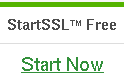
\includegraphics[width=0.1\textwidth]{images/startcomca_step1}
    \item (startcomca.com) 
\includegraphics[width=0.1\textwidth]{images/startcomca_step2_signup}
    \item (startcomca.com) Fill out the form.
    \item (your e-mail account) A verification code will arrive.
    \item (startcomca.com) Enter the verification code, click ``sign up''.
      
      The system could not install the login certificate
      automatically, you should install it manually.  Create a
      ``Private key password'' Please click here to install the
      issuing CA certificate into your browser first.  save a *.p7b
      file
      
    \item Skip to section~\ref{cert_install}
    \end{enumerate}
  \end{multicols}
\end{minipage}

\subsubsection{If you chose another certificate authority}
Simply follow the instructions on the website of the CA.  It will
generally involve filling out a form and confirming an e-mail.


\subsection{Transferring your certificate from the browser to Mail.app}\label{cert_install}
If you generated your key pair manually, skip to \fullref{import}.
Otherwise, follow the steps below to first export your key from your
browser.
\subsubsection{(Safari only) Export your key from keychain access}
Safari stores your key on your keychain instead of keeping it internal
to the browser.  To export it:

% Double-click on Keychain to open it. On the left, click on
% ``Certificates''.  Highlight the certificate to export and open File
% $\gg$ Export. Choose an
% appropriate filename (e.g. \texttt{mycert.pfx}) and directory.

\begin{minipage}{\textwidth}% This minipage inhibits page splitting
  \begin{multicols}{2}
    \begin{enumerate}
    \item Open \emph{Finder} and go to Applications $\triangleright$
      Utilities $\triangleright$ Keychain Access.
    \item Select the ``login'' keychain from the Keychains list on the
      upper left side of the Keychain Access window.
    \item Select ``My Certificates'' in the Category list on the lower
      left side of the window.
    \item On the right side of the window, a list of certificates will
      appear. Find the one that’s associated with your e-mail
      account. If there is more than one, check the expiration date
      column and select the one with the most recent date. However, do
      not select one that has a red X on its icon; such certificates
      are invalid.
    \item From the File menu choose ``Export~Items...''.
    \item Select the ``Personal Information Exchange (\texttt{.p12})''
      file format. Give the file a suitable name, and save it
      someplace safe. I suggest that you do not save it to cloud
      storage (iCloud, Dropbox, etc.)
    \item You'll be prompted to create a strong passphrase for the
      file. This will be used to secure your certificate while you
      move it. It's important that you choose a very strong
      passphrase. I recommend using a password that's at least 20
      random characters long, or a phrase made up of six or more
      random words.
    \end{enumerate}
  \end{multicols}
\end{minipage}\\[1em]

Continue on to \fullref{import}.

\subsubsection{(Chrome only) Export your key from your browser}
Follow \href{https://www.youtube.com/watch?v=n3rOEpGjrc\&start=310}{%
  YouTube video n3rOEpGjrc} (the link of which jumps you to the
relevant point in the video), or follow these steps:

\newcommand{\pwadvice}{%
  You will be prompted for a password for the backup file.  A strong
  password is important because the next step will expose the file to
  entities who could attack it.  Since this password is temporary
  (will only need to be typed on one occasion), a strong password will
  not be a burden.}
  
\begin{minipage}{\textwidth}% This minipage inhibits page splitting
\begin{multicols}{2}
  \begin{enumerate}
  \item After creating the certificate (previous section) Chrome
    presents a status bar under the address bar saying ``Successfully
    stored client certificate..''.  Click the ``\texttt{View}'' button
    on that bar.
  \item There is a pop-up which showing basic information about your
    certificate.  Switch to the \texttt{Details} tab.
  \item Click the ``\texttt{Copy to File}'' button to launch an export
    wizard.
  \item Click \texttt{Next}.
  \item You are asked if you want to export the private key with the
    certificate.  The default answer is no, but you need to click
    ``\textbf{\texttt{yes}}'', then \texttt{Next}.
  \item You are asked which format to use.  Choose \texttt{PKCS\#12},
    then \texttt{Next}.
  \item \pwadvice
  \end{enumerate}
\end{multicols}
\end{minipage}


Continue on to \fullref{import}.

\subsubsection{(Firefox only) Export your key from your browser}

\begin{enumerate}
\item Go to: menu ($\equiv$) $\triangleright$ Options/Preferences
  $\triangleright$ Advanced $\triangleright$ Certificates
  $\triangleright$ View Certificates $\triangleright$ Your
  Certificates.\\[1em]%
  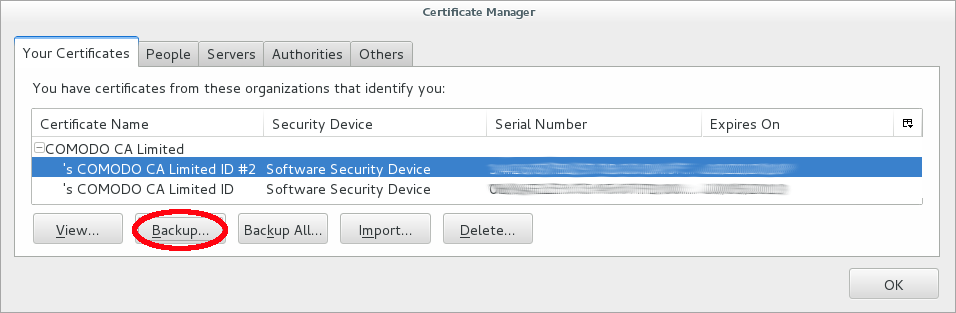
\includegraphics[width=0.7\textwidth]{images/firefox_cert_settings.png}
\item Highlight the line showing your new key.  It will be under the
  name of the CA you chose (e.g. the line under ``COMODO CA Limited''
  if you chose Comodo).
\item %\raisebox{0.6\baselineskip}{\parbox[t]{0.9\textwidth}{%
      %\begin{wrapfigure}{r}{0.7\textwidth}%
      %  \includegraphics[width=0.7\textwidth]{mailapp_firefox_cert_settings.png}
      %\end{wrapfigure}
  Click ``\texttt{Backup...}'' to export the key.
\item Save the file somewhere with a filename of your choice.  It will
  likely be given a \verb|.p12| extension.
\item\label{makebupw} You will be prompted for a password for the
  backup file.  A weak password is fine, because this backup file will
  not be transmitted or retained for long.  You will import it into
  Outlook locally, and then you will delete the backup file.
\end{enumerate}


Continue on to \fullref{import}.

\subsubsection{Export your key from browsers other than Chrome or Firefox}
\shrug\ Try to mirror the approaches above in your browser.

\subsubsection{Importing your key}\label{import}

\begin{enumerate}%\setcounter{enumi}{6}
\item Find the \texttt{.p12} file you either created manually or
  exported from a browser in previous steps.  E-mail it to yourself.
\end{enumerate}

Either follow the illustrated steps under ``Importing your certificate
into iPhone/iPad'' in
\url{https://www.comodo.com/pdf/Comodo-CPAC-iPhone-iPad.pdf},
% alternatively, and more comprehensive => http://ccit.mines.edu/UserFiles/File/ccit/security/importing_and_using_smime_certificate-web.pdf
\textbf{OR} continue with the following steps:\\
\begin{minipage}{\textwidth}% This minipage inhibits page splitting
  \begin{multicols}{2}
    \begin{enumerate}\setcounter{enumi}{1}
    \item (on your iOS device, in mail.app) open the above-composed e-mail.
      Do this on all your iOS devices.
    \item Open the file attachment by tapping it.
    \item Tap ``\verb|install|'' at the top right.
    \item Ignore the unsigned profile warning, and tap ``\verb|install|''
      two more times (or as needed).
    \item At the password prompt, enter the \emph{backup} password created
      in step \ref{makebupw}.
    \item Tap ``\verb|Next|'' at the top right.
    \item Tap ``\verb|Done|'' at the top right.
    \item (optional) The key backup file and e-mail carrying it
      may be deleted and the password may be forgotten at this point.
      There is no further use for them.  The backup file can always be
      re-created from Firefox if the key must be imported to other
      iOS devices later.
      % http://www.macwhiz.com/blog/2014/11/18/apple-s-mime/
    \end{enumerate}
  \end{multicols}
\end{minipage}\\[1em]

The new certificate will expire (see ``validity'' in section~\ref{catable}).

\subsection{Enabling S/MIME functionality in mail.app}\label{smime_enable}
Either follow the illustrated steps under ``Enable S/MIME for your
mail account'' and ``Enable signing and encryption'' in
\url{https://www.comodo.com/pdf/Comodo-CPAC-iPhone-iPad.pdf}, or
continue with the following steps:\\[-2em]%
\begin{wrapfigure}{r}{0.2\textwidth}%
  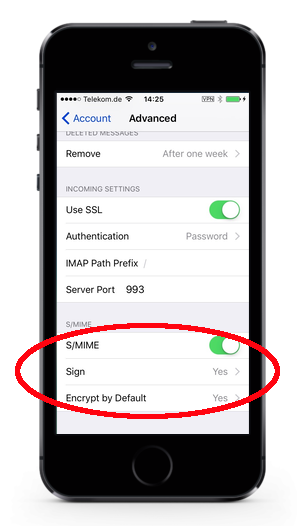
\includegraphics[width=0.2\textwidth]{images/mailapp_smime_settings_indicated.png}
\end{wrapfigure}%
\begin{enumerate}%\setcounter{enumi}{14}
\item (iOS device) go to: Settings $\triangleright$ Mail, Contacts,
  Calendars $\triangleright$ Accounts: (e-mail service provider for
  the address you created a key for) $\triangleright$ IMAP:
  Account... $\triangleright$ Advanced $\triangleright$ S/MIME.
\item enable it
\item go to: ``\verb|Sign|'' and enable it.  There will be an address under
  ``Certificates'' if the certificate installation worked earlier.
\item repeat the above step for ``\verb|Encrypt|''
\item go back: \textbf{Account} $\ll$ Advanced
\item tap ``\verb|Done|'' in the top right corner.
\end{enumerate}

\subsection{Distribute your S/MIME certificate (aka public key)}
In short: simply send an e-mail to the recipient using mail.app.  If
you created your own CA and key pair manually instead of using your
browser to subscribe to a CA, then you must also send the
\verb|ca.crt| file
that you created.\\

Detailed explanation: You have a pair of keys (these were created in
section~\ref{catable}).  One is a public key and the other is a
private key.  The public key must be sent to those who will send you
encrypted e-mail.  They will use your public key to encrypt messages
to you.  Your public key is automatically contained in the signature
of all messages you send using mail.app (because you enabled S/MIME
signing in section~\ref{smime_enable}).

So to distribute your public key, simply send the other party an
e-mail from mail.app, which need not be encrypted.  They can then
extract your public key from your signature (which is composed as an
attached file named ``\verb|smime.p7s|'').

\section{Prep to send encrypted mail% or verify signatures on received mail
}
Before you can send someone an encrypted message, you need their
S/MIME certificate (public key).  Follow section~\ref{smime_enable} if
you haven't already done so, but instead of configuring the e-mail
service provider for your own key, choose the e-mail service provider
you will send the encrypted messages from (if different).  Then follow
the next section (\ref{import_cert}):

\subsection{Importing the S/MIME certificate of another
  party}\label{import_cert}
\begin{minipage}{\textwidth}
  \begin{multicols}{2}
    \begin{enumerate}
    \item Ask the other party to send you a signed message.
    \item %\raisebox{0.6\baselineskip}{\parbox[t]{0.9\textwidth}{%
          Open the signed message in mail.app.  Successfully signed
          messages have a blue ten-point star with a check in the center,
          which appears to the right of the senders
          address. E.g. \raisebox{-0.8\baselineskip}{%
            
\includegraphics[width=0.2\textwidth]{%
              images/mailapp_smime_signed_checkmark.png}}
          
    \item Tap the \emph{From} address.
    \item Tap ``\verb|View Certificate|''.
    \item Tap the ``\verb|Install|'' button.
    \item Tap ``\verb|Done|'' on the top right corner.
    \end{enumerate}
  \end{multicols}
\end{minipage}\\[1em]

Now you can send encrypted messages to the sender.

\end{document}

% Extra notes for protonmail users:
% 
% 1) click on "SETTINGS" at the top.
% 2) click on "Keys" in the left frame
% 3) click on "Public Key" under the "Download" column
% 4) choose "save file", and save it to a place where you will remember (for the next step)
% 5) compose an e-mail to me, and attach that file you just saved

% some useful info here: http://www.macwhiz.com/blog/2014/11/18/apple-s-mime/#Part_One:_Export_the_certificate_from_your_Mac
